\chapter{Requirement Analysis}
	
Before designing a piece of software, it is important to hold good understanding of the project requirements. In this chapter a number of functional and non-functional requirements will be listed covering all the aspects of the future project.

\section{Target Audience}
\label{sec:targetaudience}
	
The intended users of the application developed will be people with interest in football. More specifically, people interested in predictions of football results and football betting. With this in mind, the age range of potential users will be 18 and up.

\section{Target Audience Questionnaire}
\label{sec:targetaudiencequestionnaire}
The target audience research aims to gather information on how...
Due to the spread of target users, an electronic questionnaire was used to collect the results. A full break down of the questions asked and the answers received can be found in the appendices, reference X.

\section{Researching the Potential competitors}
\label{sec:researchingcompetitors}
Before gathering the project requirements, it is good practice to conduct research on what current websites are already available to football fans. The research can be a source of inspiration and would also help to avoid possible design mistakes. During the analysis, it is important to attempt to understand the main purpose of the analysed applications, as well as the way they present information and communicate with their users. \par

    
This section is concerned with websites that can be useful for predicting football results. In our context, these are the online sources of information a football punter would turn to before making a betting decision unless the decision is based solely on punter's intuition. In general, several different types of such websites can be found online, namely:\par
		
\begin{enumerate}
	\item Sports news websites
	\item Football statistics websites
	\item Websites of betting providers 
	\item Communities 
	\item "Black-box" prediction applications
\end{enumerate}

This section of the report looks at one or two examples of each of the categories presented above, analysing the weak and strong points of the chosen website and discussing usefulness of the whole category from the point of view of a footaball punter.
	
	\subsection{Sports news websites}
	\label{subsec:sportsnewswebsites}

This category represents football news websites. Into this category belong both general sports websites having a football section and football news websites, for example:
	
\begin{itemize}
	\item BBC Sport - \url{http://www.bbc.co.uk/sport}
	 \item The Guardian Sport News - \url{http://www.theguardian.com/uk/sport}
	 \item Sky Sports - \url{http://www.skysports.com/}
	 \item 	The Times Sport section - \url{http://www.thetimes.co.uk}
	 \item Football365.com - \url{http://www.football365.com}
	 \item Goal.com - \url{http://www.goal.com}
\end{itemize}

The sports news websites aim to present the news alongside the essential football statistics. The information is usually not as detailed as on the football stats websites, however the very latest football news compensates for this drawback. Each of the \emph{news} websites named above (BBC News, The Guardian, Sky Sports) have a football section that presents the reader with the combination of football news and stats.  One of the most popular football news websites is BBC Sport Football.
	
	\subsubsection{BBC Sport Football}
	\label{subsubsec:bbcsportfootball}
	
BBC Sport Football is a brilliant news website. It offers very neat and simple interface and does not overwhelm the reader with irrelevant graphics. Although, it almost looks too minimalistic, the user can still find the most important information about football teams and players. The website provides authomatically updated live scores accross all featured football leagues.\par


BBC Sport has a very impressive news coverage of both major and minor British football leagues, as well as the main european leagues. It can also take pride in high quality writers (journalists) contributing to the website. An interesting feature is videos embedded in the webpage.\par


As already mentioned above, the main drawback is that the stats are kept to a bear minimum. This can be a problem for a passionate football fan that wantс to analyse the  details of the game from all possible angles. However, for a purposes of a punter this level of statistics should be sufficient.\par
	
\begin{figure}[H]
	\begin{center}
		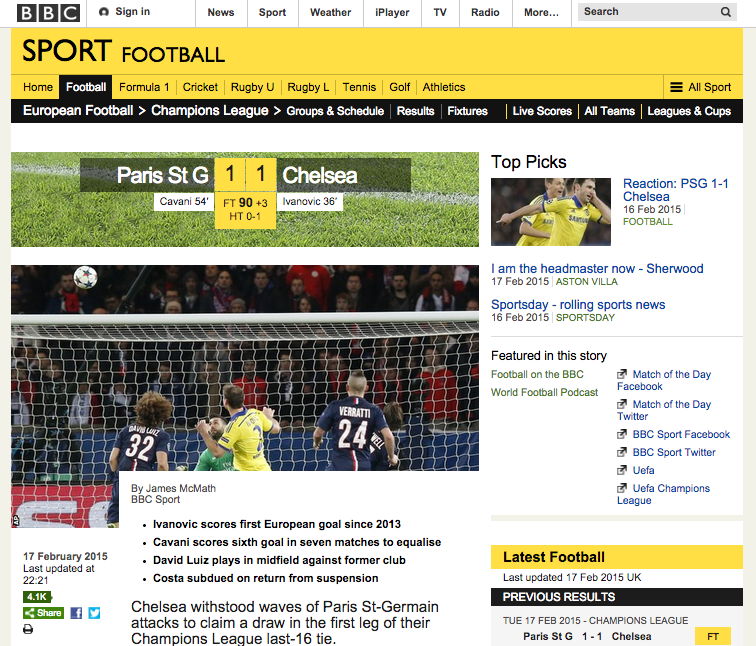
\includegraphics[width=.60\linewidth,natwidth=610,natheight=642]{req/images/bbcsport.png}
		\caption{BBC Sport - Football section} \label{fig:using:bbcsport}
	\end{center}
\end{figure}
		
\subsection{Football statistics websites}
\label{subsec:footballstatswebsites}
	
Football statistics websites focus on detailed statistics and analysis on football matches, teams and players. These are some examples of such websites:
			
	\begin{itemize}
		\item WhoScored - \url{http://www.whoscored.com}
		\item Squawka - \url{http://www.squawka.com}
		\item WhoIsInjured 	- \url{http://whoisinjured.com}
	\end{itemize}

	\subsubsection{WhoScored}
	\label{subsubsec:whoscored}
	
Among all football stats websites I have analysed, WhoScored is one of the most impressive ones. It has a lot of statistics, but most of it seems to be quite relevant. The website is extremely well designed, and its navigation is intuitive. The website is offering statistics and deep analysis on the major European divisions, as well as providing data on over 500 leagues and 15,000 teams. As to the data source, the website is supported by Opta, the biggest and a very reliable live sports data company standing behind BBC Sport, Sky Sports, etc.\par


The way "WhoScored" presents information on particular matches to the user can be very inspirational for this project. \par

\subsubsection{Squawka}
\label{subsub}
	
Squawka is another websites worth looking at. It is an award-winning application for football fans that uses real-time data visualisations to explain the game. The main idea behind is to help users to understand the game. 
		
\begin{figure}[H]
	\begin{center}
		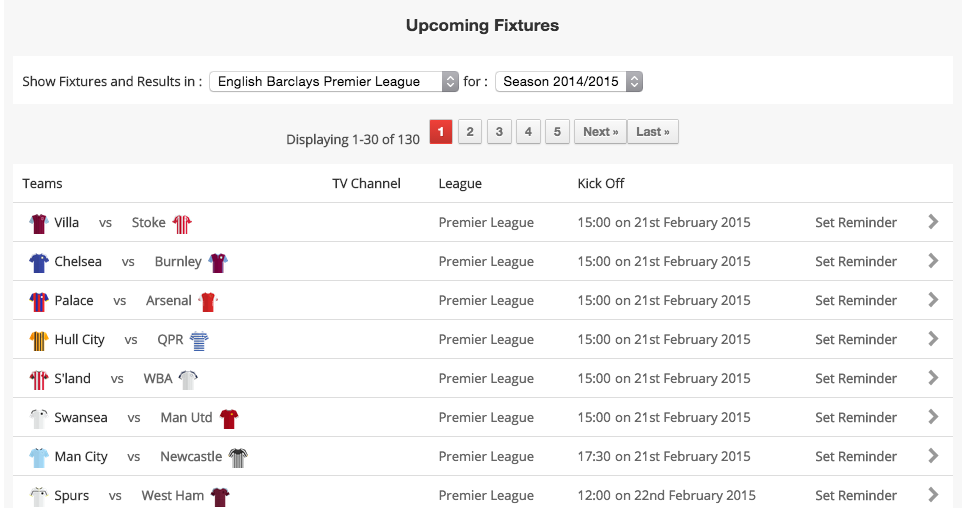
\includegraphics[width=.60\linewidth,natwidth=610,natheight=642]{req/images/squawka.png}
		\caption{Squawka} \label{fig:using:squawka}
	\end{center}
\end{figure}
	
From a visual point of view, Squawka has a nicely designed, pleasant interface. However, it is a little bit heavy on the client-side (Javascript), which contributes to sometimes slow performance. Another downside of the website is an extensive amount of adverts that distracts the user form the main content.\par
	
\subsection{Websites of betting providers}
\label{subsec:websitesofbettingproviders}
	
In this category can be named many websites.
	
	
\subsection{Communities}
\label{subsec:communities}
	
Communities is an category of the websites with an interesting idea behind. These websites are specialised social networks for sports fans and punters. There are two websites in this category:
	
\begin{itemize}
	\item OLGB Betting Community - \url{http://www.olgb.com}
	\item Vital Football News and Fans community - \url{http://www.vitalfootball.co.uk}
\end{itemize}
	


	
\subsection{Black-box prediction applications}
\label{subsec:blackboxapplications}
	
	http://www.predictz.com/predictions/europe/champions-league/609828/
	http://www.vitibet.com
	http://www.forebet.com/en/
	small prediction tool at goal.com:
	http://www.goal.com/en-gb/match/psg-vs-chelsea/1974582?ICID=FX


Firstly, there are websites containing detailed football statistics and its analysis. Some of them may also attempt (not nessesarily) to make predictions based on these statistics, however, this is not the main purpose of such websites. among \par

	  	
After having analysed the above websites from various categories, I came to the following conclusion. A well-chosen combination of several websites will be definitely able to provide enough information to make a thoughtful betting decision. \par

 		
Most punters would have their own football betting system (betting strategy). Although even the best system cannot guarantee success, it can greatly increase the prospects of making a profitable bet. Therefore, when predicting football match result, a potential punter will have to make a small research each time. The aim of such research would be to make note of the relevant statistics for the teams involved in the game (depending on the "input variables" of the betting system), for example previous results for both teams, their performance at home and away, players statistics (injuries, suspensions, transfers), recent change of team managers, etc. The problem is that many football stats websites offer way too detailed information for this purpose, therefore the relevant stats needs to be "hand-picked" from several sources for each match. \par

 	
The application will attept to put all the relevant statistics in one place and break the information down into logical "prediction modules". In addition, the application will enable users to pick the input variables and assign them a weight of user's choice, representing the importance of the input variable for the match results prediction.\par

 
\section{Requirement Analysis}
\label{sec:requirementanalysis}

Computer Systems life cycle consists of five phases: Requirements and Analysis, Design, Implementation, Testing and Evolution. Then, after Evolution, the cycle can start again with an additional set of requirements. Therefore, the Requirements analysis is a crucial part of the project and the cornerstone of the software development life cycle. Requirements analysis involves gathering information in order to meet customer needs and defining what the future application is expected to do. This phase is especially important in the real world environment, when developing an application for a customer. In this case, clarifying the requirements in the early stages of the project would help to ensure that both sides understand and agree on the feature set of the future application. \par


Although it is not very likely that requirements for this project will change during the development process, defining requirements can be very beneficial. The detailed requirements analysis will aid understanding how different parts of the project are expected to interact with each other, as well as how the application will communicate with its users.\par


For better transparency project requirements have been split into functional and non-functional requirements.\par


Before outlining project requirements, I would like to start with some definitions relevant to the whole project.\par

\subsection{Definitions}
\label{sec:definition}

\textbf{Application Football League} - in order to reduce unnecessary complexity at this stage of the project, the application will be only supporting one league (Premier Barclays League)

\textbf{Matches Overview} – a list of upcoming and played matches presented on the main page of the application

\textbf{Dashboard} - an interface available to authorised users, containing a list of played ("archived") and upcoming matches saved by the user

\textbf{Prediction Module} – my own term, standing for blocks of football statistics for each of the playing teams (for example, league position), that are evaluated against each other and based on the result of such evaluation, a match prediction (in favour of one of the teams) is made. Application calculates "prediction value" for each of the modules. 

\textbf{Match Result Prediction} - to calculate a match result prediction, each prediction value is first multiplied by its weight. The weights would be different for each user unless default system settings are being used). Then, all of the weighted values are added together and based on this value a prediction is made.

\textbf{Default System Settings} - application has a set of default weights for each prediction module. These weights are used in the prediction calculation by default. 
 
\textbf{Default User Settings} - each user of the application can save a set of prediction weights that are different from the default system settings. From the moment these weight are saved, they will be used by default for each match committed by the user. 

\textbf{Match Specific Prediction Settings} - each user of the application can also save a set of prediction settings specific for only one match. 

\textbf{Match result} - "Home Win" in case of the win of the hometeam, "Away Win" in case of the win of the awayteam, "Draw"for the draw


\subsection{Functional Requirements}
\label{sec:functionalrequirements}

Functional requirements describe the behaviour of the application in terms of its functionality. These are the "must have" functions of the application addressing the business targets that application must satisfy. Good functional requirements must be concise, complete and unambiguous.\par
 
In order to add structure to the design and development process, the project was broken down into high level features of the future application. The functional requirements are grouped by the functionality related to those features.\par

\subsubsection{General Web Application Requirements }
\label{sec:generalwebrequirements}

These are the requirements related to the basic functionality of the web application, such as account registration, login and account management.\par

\begin{itemize}
  	\item The application should allow users to register and create a new account with the application
  	\item User will be able to register using a standard web form
  	\item For the registration purposes user will provide a valid email address and a password
  	\item User will confirm a password in a separate input field
  	\item After a successful registration application will send an email containing a confirmation link to the user
  	\item On a successful confirmation of an email address, user will be successfully registered
  	\item In case of any technical problems with the initial confirmation email, the application will be able to issue a new email and send it to users on their request
	\item The application should allow users to sign into their accounts using a standard web form
	\item When signing in, user should provide valid credentials, otherwise an application will throw a validation error
	\item The application will allow users to manage their account by changing personal information  (for example, location, favourite football team)
	\item The application will allow users to change the email address associated with their account
	\item The application will provide an option to change user password for security reasons
\end{itemize}

\subsubsection{Matches Overview}
\label{sec:matchesoverviewrequirements}

Below are the requirements relating to the matches overview.\par

\begin{itemize}
	\item On the main page of the application user will be presented with a list of upcoming matches for the current season in the league
	\item User will be also able to view a list of played matches and switch between upcoming and played matches using navigation tabs
	\item For each of the unplayed matches user should be able to navigate to the match page and see more details about the match
	\item From the main page user will be able to save any unplayed match to the dashboard
	\item For each of the played matches user will be able to navigate to the match page and see more details about the played match
\end{itemize}

\subsubsection{Prediction}
\label{sec:prediction}

The predicted outcome of a football match in the application will be calculated after evaluating several factors that can influence the match result. An example of such a factor could be a previous match result, league position of each team or a team's performance at home. Each of those factors is represented by an equivalent "prediction module" in the match view. These are the requirements related to the prediction of the overall match result. \par
	
\begin{itemize}
  \item To calculate prediction values for each module, application uses default system settings in absense of default user prediction settings or match specific settings
  \item Application uses default user prediction settings in absence of match specific settings
   \item Application uses match specific settings in case user set them for this match
 \end{itemize}

\subsubsection{Upcoming Match View}
\label{sec:generalpredictionrequirements}

Users should be able to view detailed statistics of the upcoming match. These are the requirements related to this functionality.\par

\begin{itemize}
	\item The information presented in the unplayed match view will be divided into two major sections: prediction modules and additional information 
	\item For an unplayed match user should be able to see a set of prediction modules
	\item Each module should contain relevant piece of football statistics
	\item For each module it should be clear which team is a winner for the module and what is a probability for this outcome if the prediction wuld be based solely on this prediction module
	re will be several prediction modules and the football information for each team
	The details will include statistic data for each of the playing teams, such as team standings, results of 6 previous matches, results of previous 6 matches played at home, results of previous 6 matches played away, results of previous meetings with the opponnent within current season. 
	\item from the prediction module user can see stats of the website population
\end{itemize}

\subsubsection{Played Match View}

After the game has been played, the application will offer prediction statistics and some feedback to the user. Hopefully, this will allow users to compare their betting strategy with the fellow punters and analyse their own betting settings. These are the requirements related to the played match view.

\begin{itemize}
	\item
\end{itemize}


\subsubsection{Dashboard}
\label{sec:dashboardrequirements}

Dashboard is a key view of the application.\par

The idea behind the dashboard in this application is similar to online shoppping experience: user saves an item to the shopping basket and from the basket can submit a purchase or cancel it. In our case, user browses through the matches overview and save matches to the dashboard for a latter review. The requirements outlined below describe the dashboard functionality in more detail.\par

\begin{itemize}
	\item from the overview of the matches on the main page, user can add a match and save it to the dashboard
	\item user can delete matches from the dashboard
	\item user can override the system's recommended prediction modules weights (called "betting system settings") using the" betting system" tab in the dashboard. 	Any next match saved to the user dashboard will be shown with these user default betting settings. 
	\item user can override the user default betting settings and have different betting  settings for each saved match. User can save a match with the new weighting percentage.
	\item After completing the betting settings, user can “commit to bet” a saved match. After that match betting settings cannot be changed.
	\item If the match is saved in the user dashboard and it changes its status from "unplayed" to "played", application will evaluate user's commit and estimate whether user won a virtual bet or not based on the actual match result. 
\end{itemize}


User can “commit to bet” a match 
Committed games are marked in the dashboard (red dot)
Played games are marked in the dashboard (grey font)
Once user committed games has started (observer, onchange on a filed), it should indicate the winnings and write to db
Fix the kits

\subsection{Non-functional Requirements}
\label{sec:nonfunctional}

Non-functional requirements specify how the system is going to perform.\par

\subsubsection{Testability}
The application should be testable – the behaviour of the application should be verifiable through a suite of automated tests. 
A set of test cases will be written for the application, testing features such as logging in, account registration, integration with third-parties API used in the application, as well as various scenarios of database models interactions. In addition to these tests, the business logic in the match prediction must also be predictable, consistent and testable. 


Maintainability
Scalability
Documentation
Performance
Responsiveness
Usability
Usability means how easily can users learn how to use an application. The key would be to reduce an effort to understand 

\subsubsection{Security}
The nature of the application requires from user to provide some confidential information. Users need to be assured that the confidential details remains secure, and that the system is protected against XSS, CSRF and SQL injection attacks.


graceful degradation?
accessibility security


\section{Overall Architecture}
Provide a list of all the chapters within the thesis and a brief summary of the content.

\textbf Design of an application a a whole, overall design (just boxes and lines)
\textbf Architectural diagram (overview) (aosabook.org/en/moodle.html -example), quite high level


\section{Choice of Third Parties API}
\label{sec:thirdpartiesapi}
	
	After analysing the functional requirements, it became apparent that this type of application will need the latest football data in order to operate correctly. The easiest way to load such data into the application would be to integrate the application with a third party API. The process of finding an appropriate API for the project will be described in this section. 
	
	After brief research, one thing became apparent. Live football data is a very desirable product and therefore it is not easy to find free of charge live football data API.  The key problem is that the data the application needs has to be very recent. Real-time data in particular is very expensive, because of its use by the gambling industry for betting on various markets as the games are going on. It is much easier to find free historical football data.  
	
	This is a (not complete) list of API providers that I researched about.
	
	\begin{itemize}
		\item Optasports.com (http://www.optasports.com)
		Opta is an industry leader. It provides a wide range of XML feeds covering many sports. The feeds include fixtures and results, live scores, live player stats and many more. Data provided by Opta is very reliable and is used by top-notch clients, such as BBC Sports, BT Sport, Sky Sports, as well as many betting providers and newspapers.
		
		\item Openfooty (http://www.footytube.com/openfooty/service.php) 
		Openfooty is an interesting project with very detailed API documentation. However, a quick look at the developer forums shows a stale community and many questions about why no one seems to actually be able to get a developer key.	Unfortunately, I also did not manage to obtain a key for this API.	
		
		\item football-api (http://www.football-api.com)
	is a paid API service but does offer the English Premier League endpoints for free (demo use). The API will restrict by IP addresses and limit calls based on your package. 	Includes endponts for Competitions, teams, standings, live scores, fixtures and commentaries. See the pricing page.		
		
	\end{itemize}
	
However, there can be found many high quality APIs that are not for free. how I came to choose the API I am using in the application


\section{Project Plan}
The project progress timetable is presented in the Gantt diagram below. I found it appropriate to set In general, my two main milestones will be completing the first prototype of the application before the Christmas break and completing the second prototype by the end of April, 2015 (this includes all the testing and bug fixes). 

The first prototype will have implemented most of the basic features of the application (my development part is broken down into features - viz. the Gantt diagram). The second prototype is the final version of the application; it will include all the planned features and the graphical design. I will try to make an even progress on the report throughout the whole time available, as it can be seen from the diagram.


\section{Conclusion}
A short conclusion summarising the chapter.
